\documentclass{beamer}
\beamerdefaultoverlayspecification{<+->}
\usepackage{soul}

\usetheme{Berlin}

\title{Aplicativo web de auxílio à navegação aérea}
\author{Antenor Barros Leal}
\institute{Departamento de Informática \\ PUC-Rio}
\date{Dezembro 2024}

\begin{document}

\begin{frame}
    \titlepage
\end{frame}

\begin{frame}{Outline}
    \tableofcontents
\end{frame}

\section{Introdução}

\begin{frame}{Introdução}
    \begin{itemize}
        \item Flight Bag
        \item Electronic Flight Bag
        \item Simulação de voo
        \item AISWEB, METAR-TAF, SIGMET
    \end{itemize}
\end{frame}

\begin{frame}{UI}
    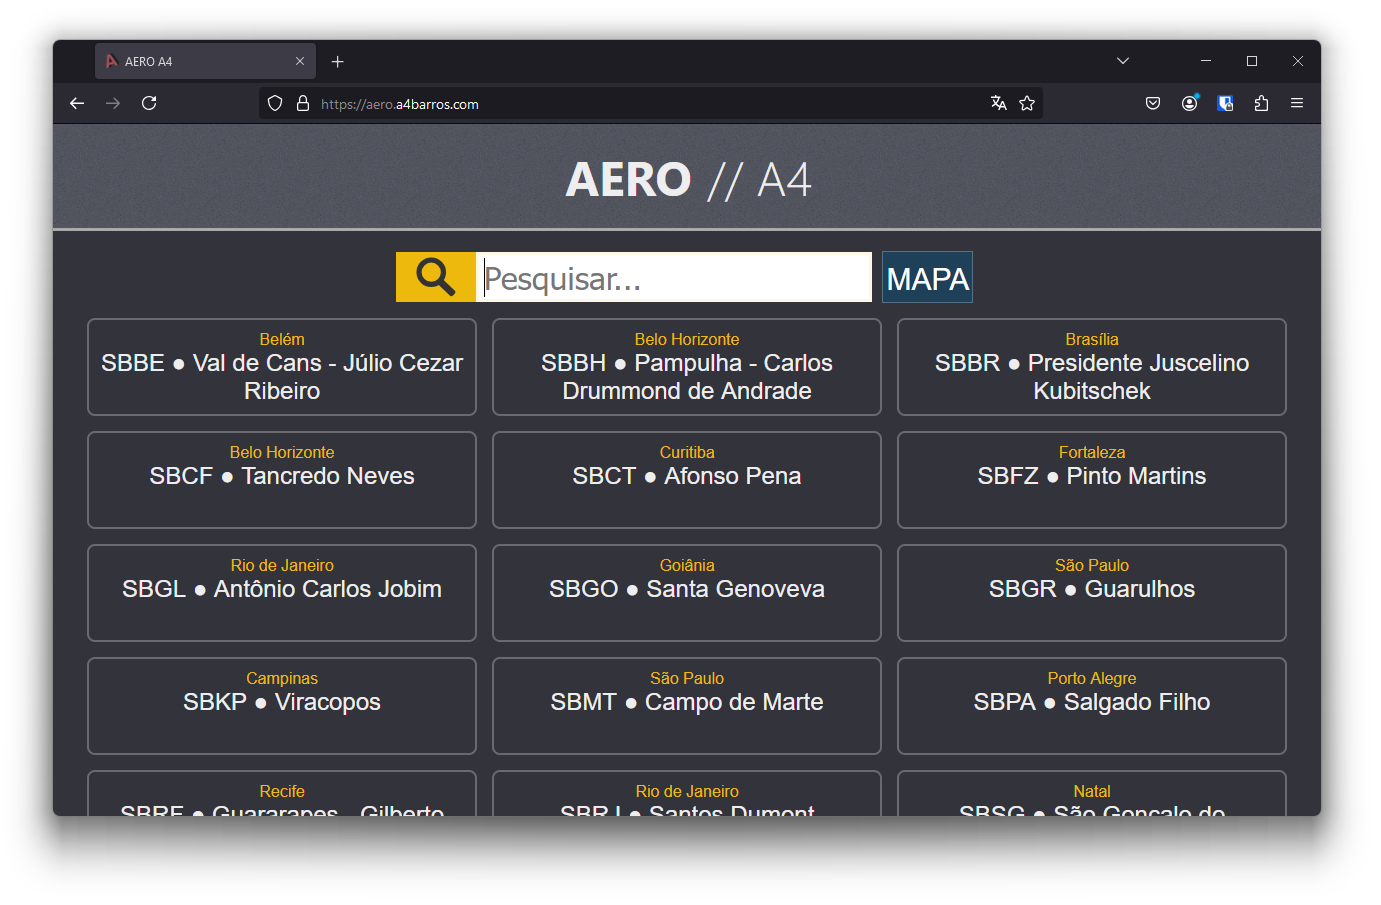
\includegraphics[width=0.7\linewidth]{img/UI.png}
    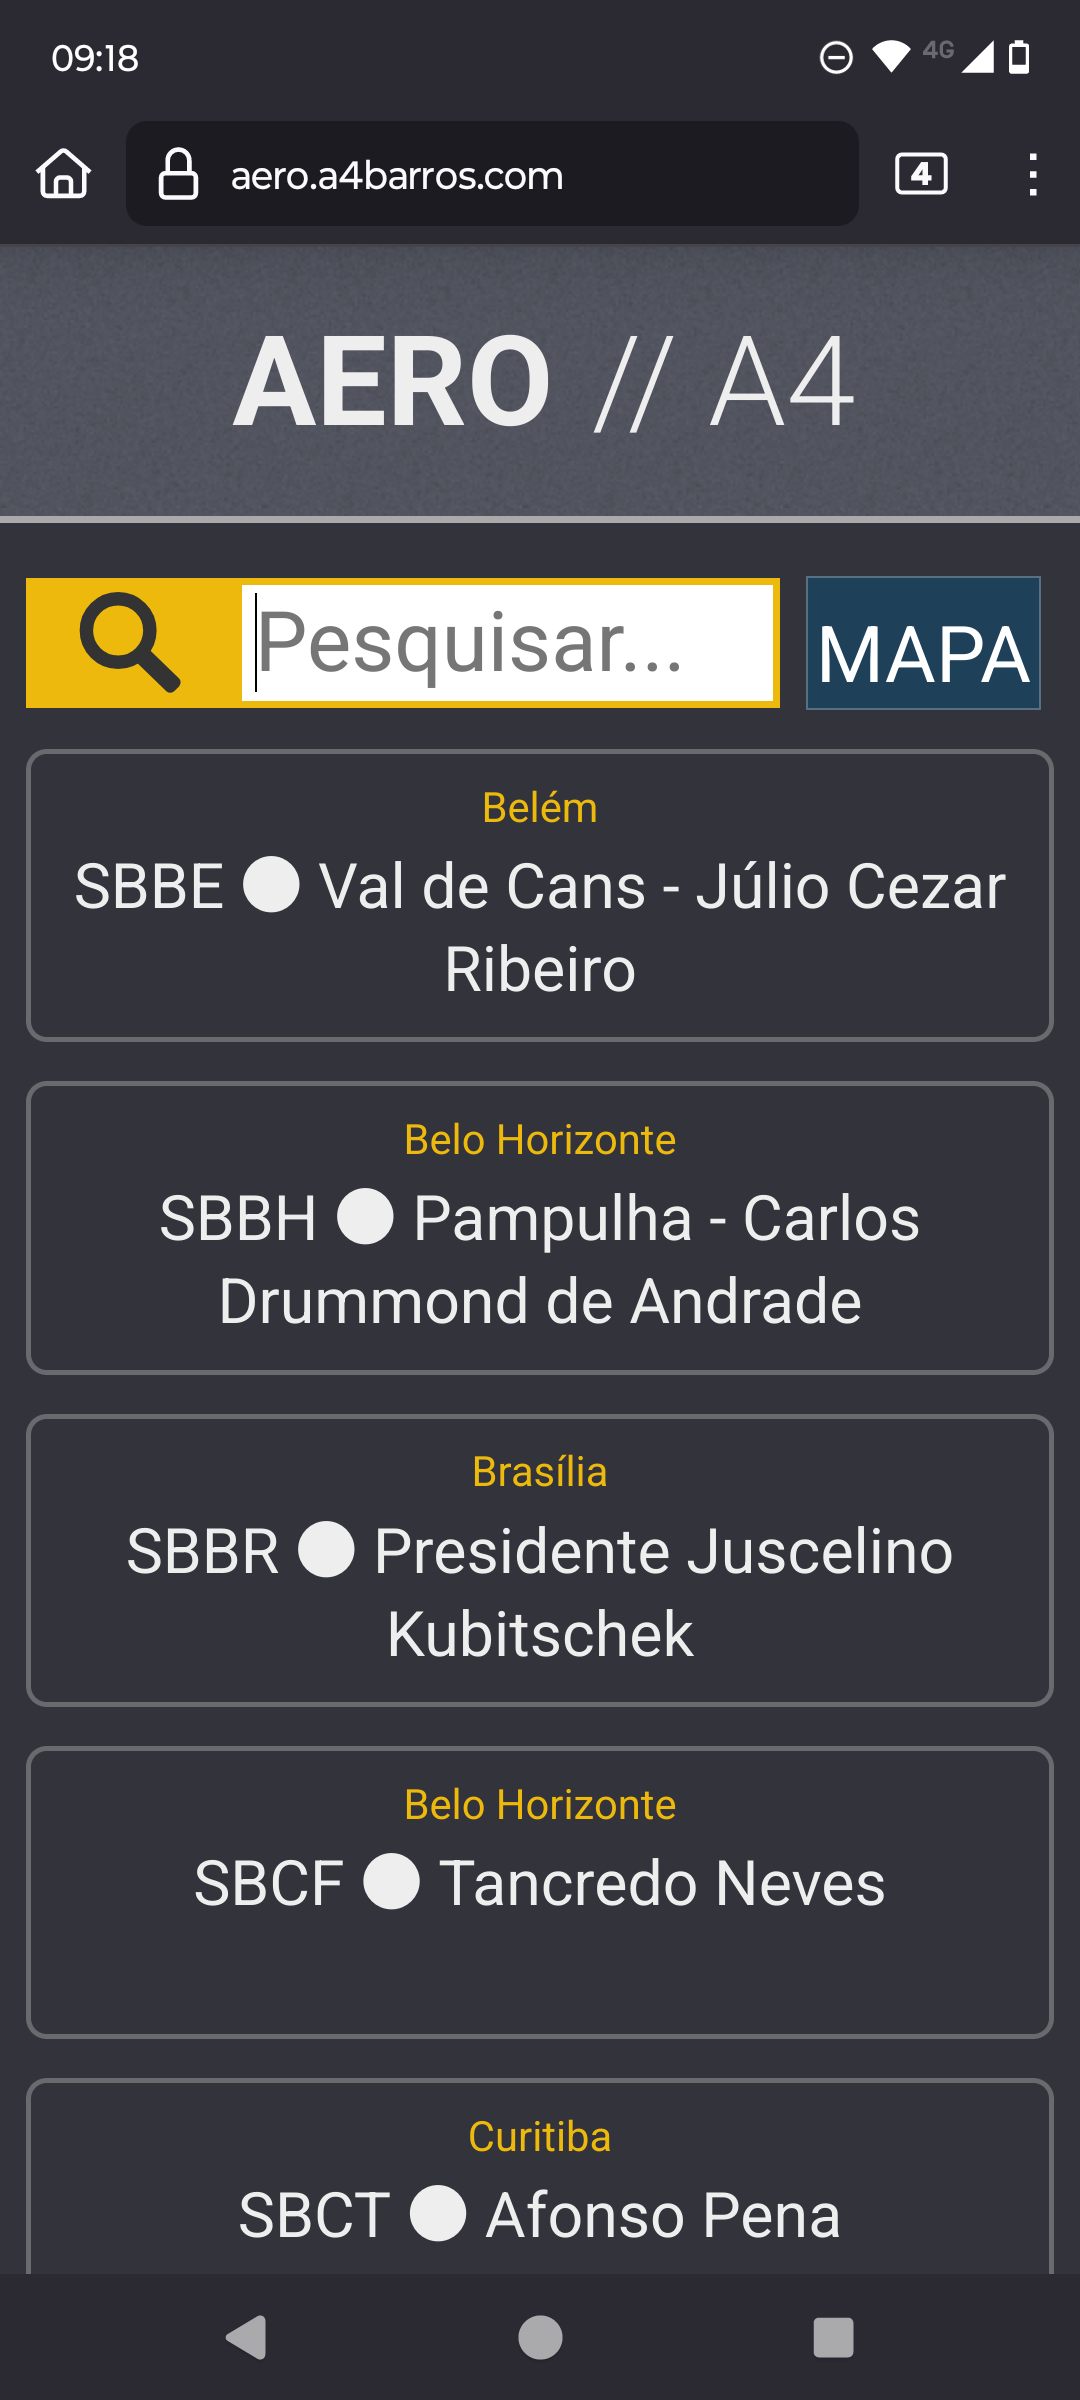
\includegraphics[width=0.2\linewidth]{img/UI_mobile.png}  
\end{frame}


\section{Arquitetura}

\begin{frame}{Servidor}
    \begin{figure}[ht]
        \begin{center}
        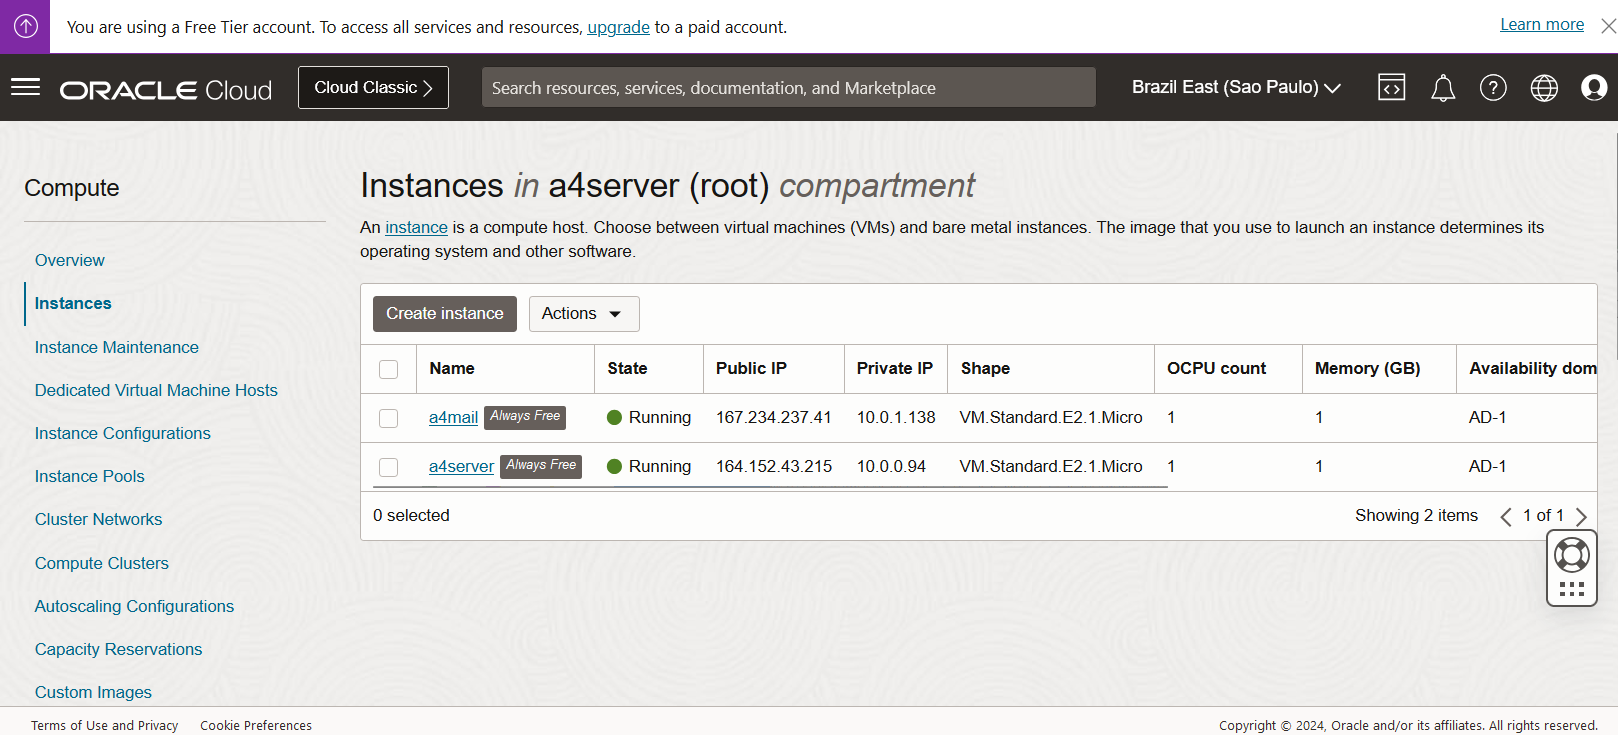
\includegraphics[width=0.9\linewidth]{img/oracle.png}
        \label{fig:UI}
        \end{center}
    \end{figure}
\end{frame}

\begin{frame}{Arquitetura}
    \begin{itemize}
        \item Docker/Docker Compose
        \item Banco: MariaDB
        \item Backend: \st{Flask} FastAPI
        \item Frontend: Jinja2
        \item Observabilidade: GoAccess
        \item Outros subdomínios
    \end{itemize}
\end{frame}

\begin{frame}{Uso de rescursos}
    \begin{itemize}
        \item 500 acessos simultâneos (usando Locust)
    \end{itemize}
    
    \begin{figure}[ht]
        \begin{center}
        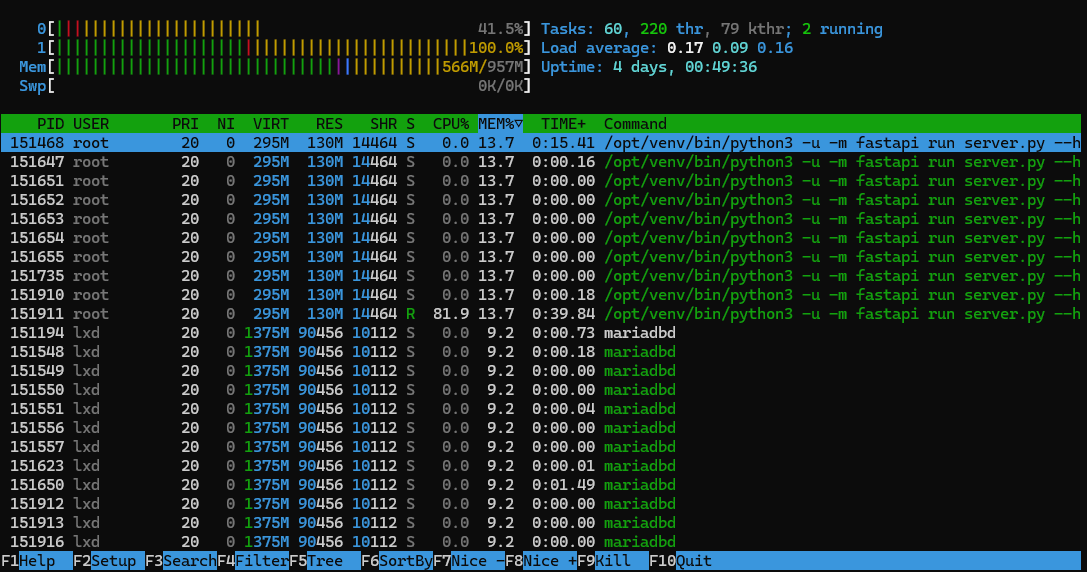
\includegraphics[width=0.8\linewidth]{img/server-500-acessos.png}
        \label{fig:arquitetura}
        \end{center}
    \end{figure}
\end{frame}

\begin{frame}{Diagrama da arquitetura}
    \begin{figure}[ht]
        \begin{center}
        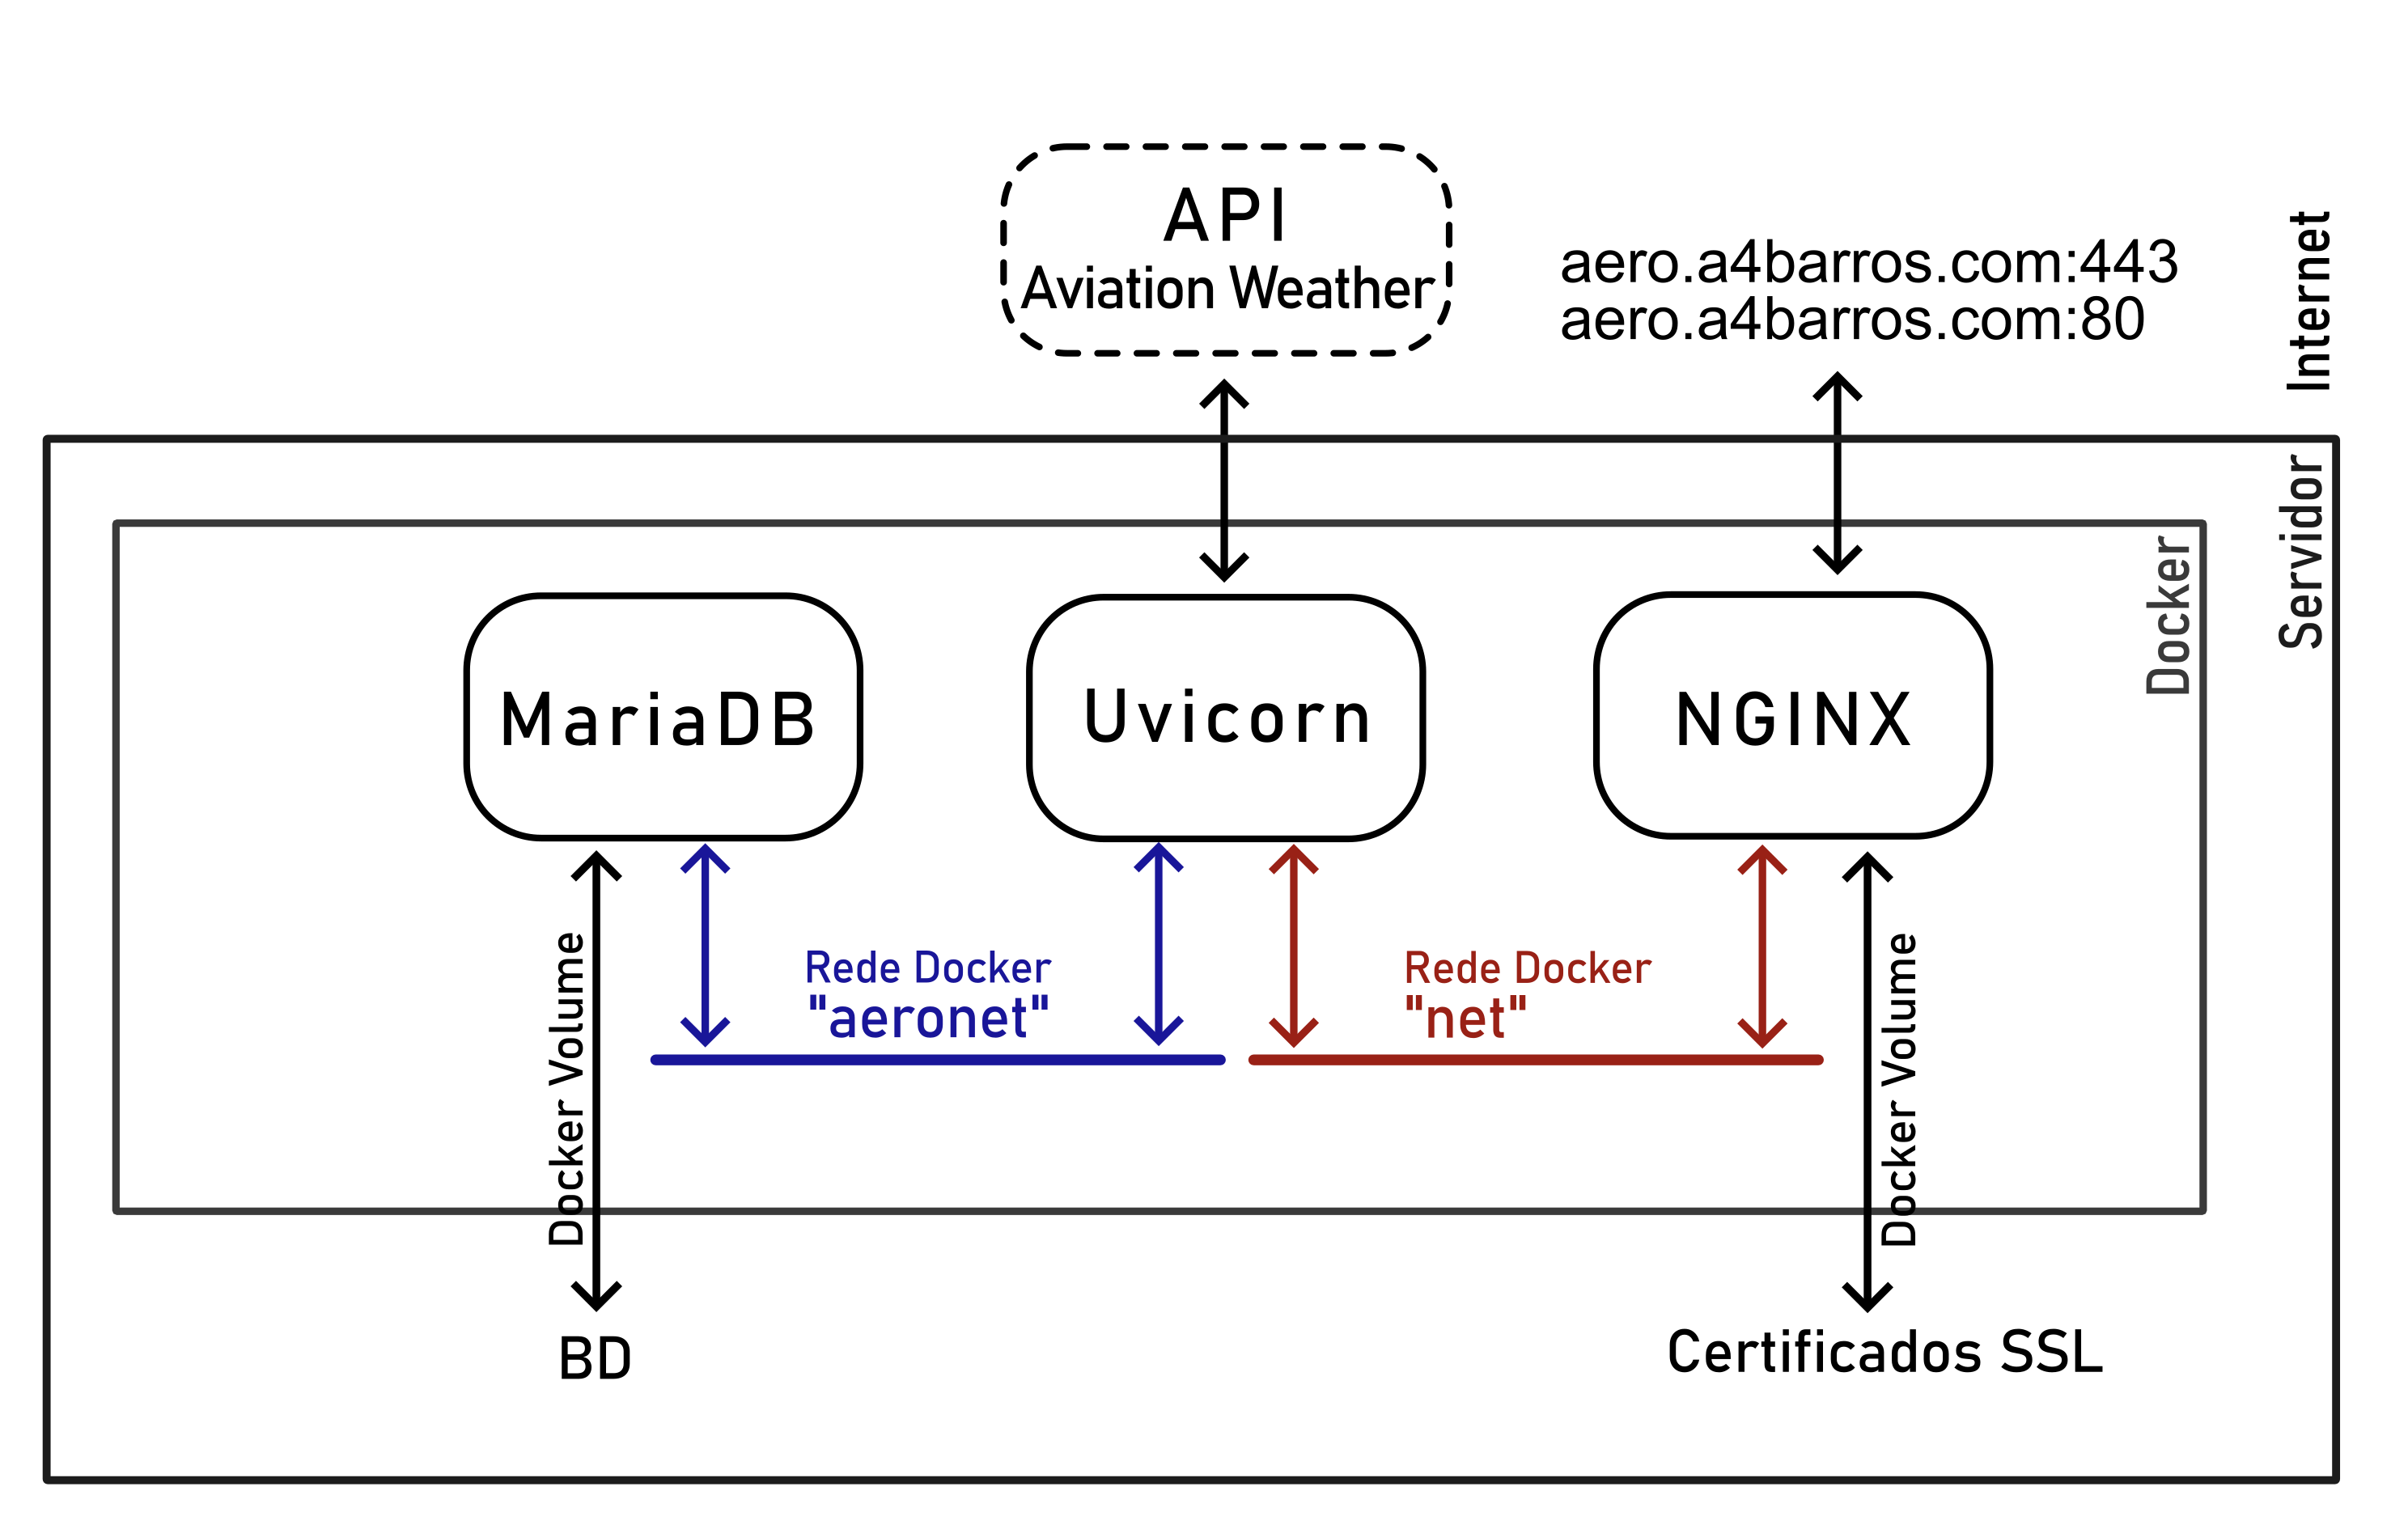
\includegraphics[width=0.8\linewidth]{img/diagrama-arquitetura.png}
        \label{fig:arquitetura}
        \end{center}
    \end{figure}
\end{frame}

\begin{frame}{Diagrama de tempo}
    \begin{figure}[ht]
        \begin{center}
        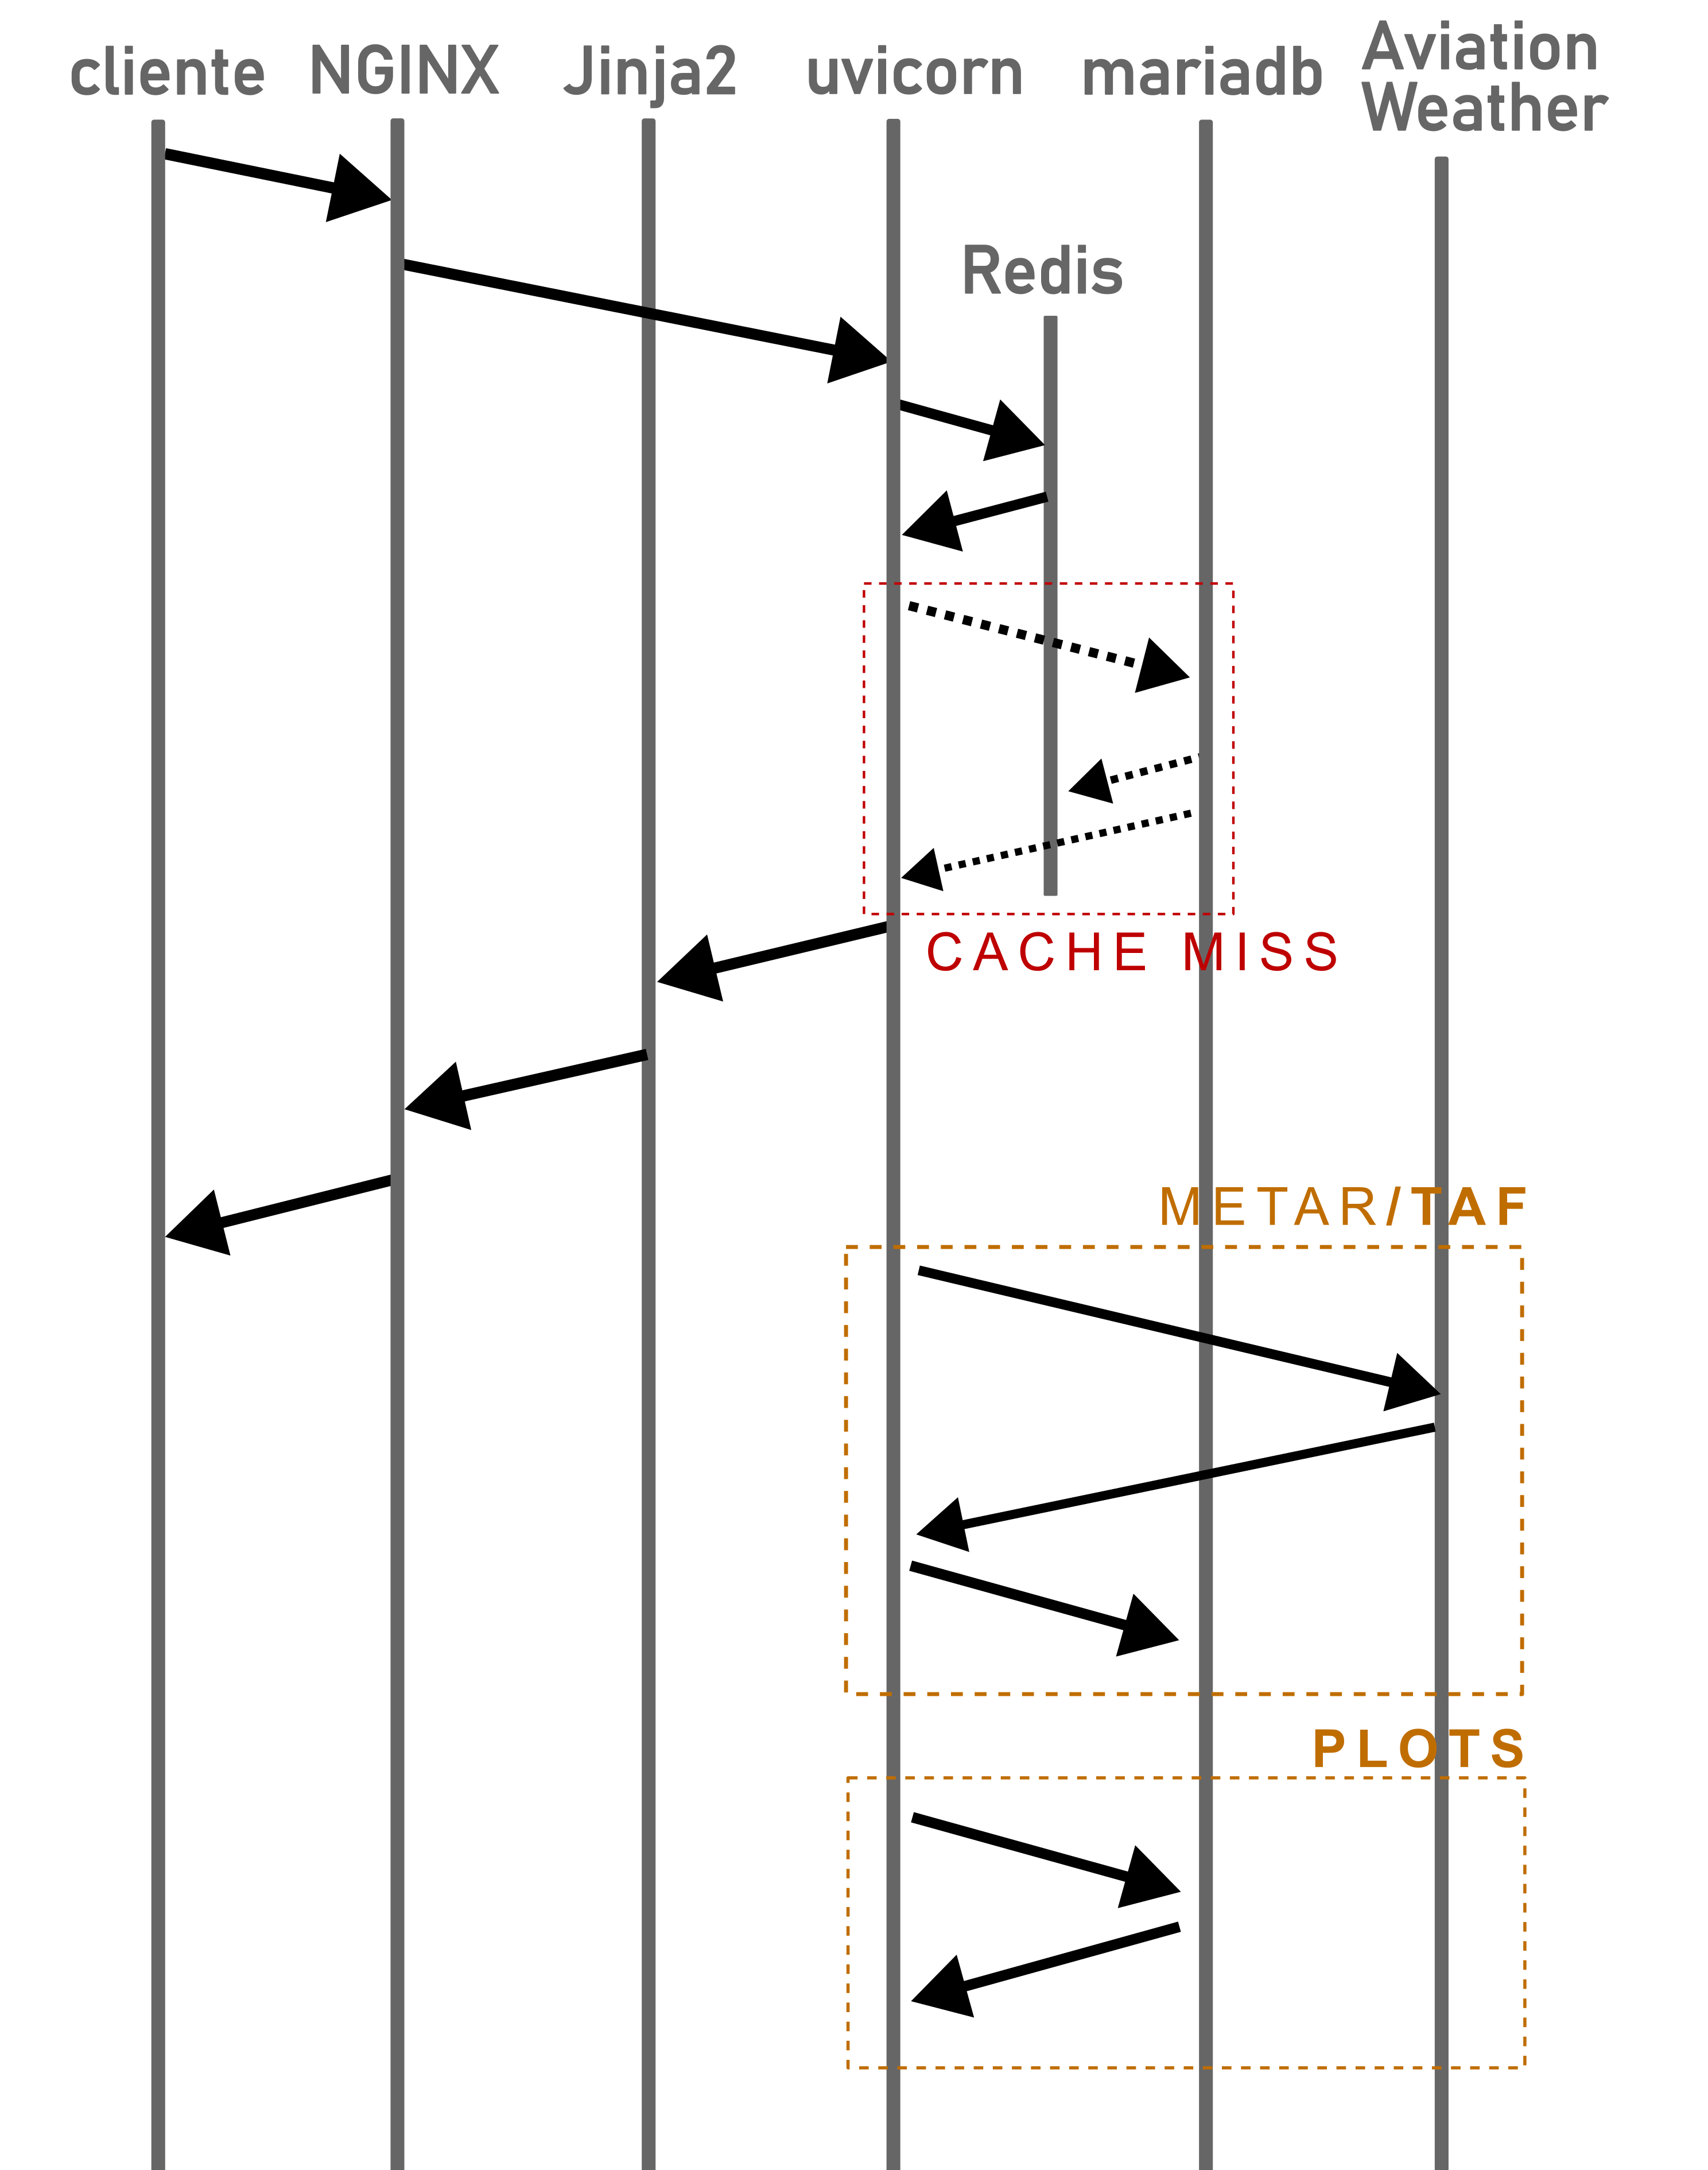
\includegraphics[width=0.4\linewidth]{img/diagrama-tempo.png}
        \label{fig:arquitetura}
        \end{center}
    \end{figure}
\end{frame}


\section{Projeto}

\begin{frame}{Tabelas}
    \begin{figure}[ht]
        \begin{center}
        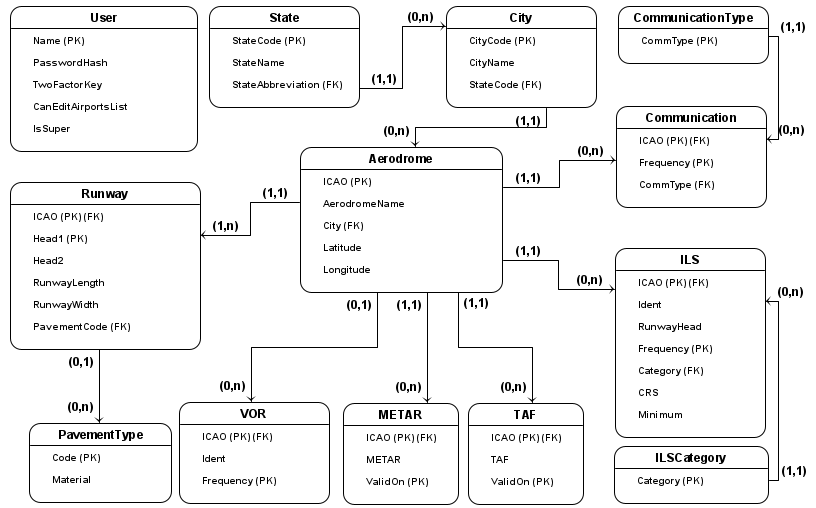
\includegraphics[width=0.8\linewidth]{img/ERAero.png}
        \label{fig:arquitetura}
        \end{center}
    \end{figure}
\end{frame}

\begin{frame}{METAR}
    \centering
    \small{\texttt{221300Z 04008KT 9000 FEW020 BKN100 30/23 Q1012}}
    \begin{figure}[ht]
        \begin{center}
        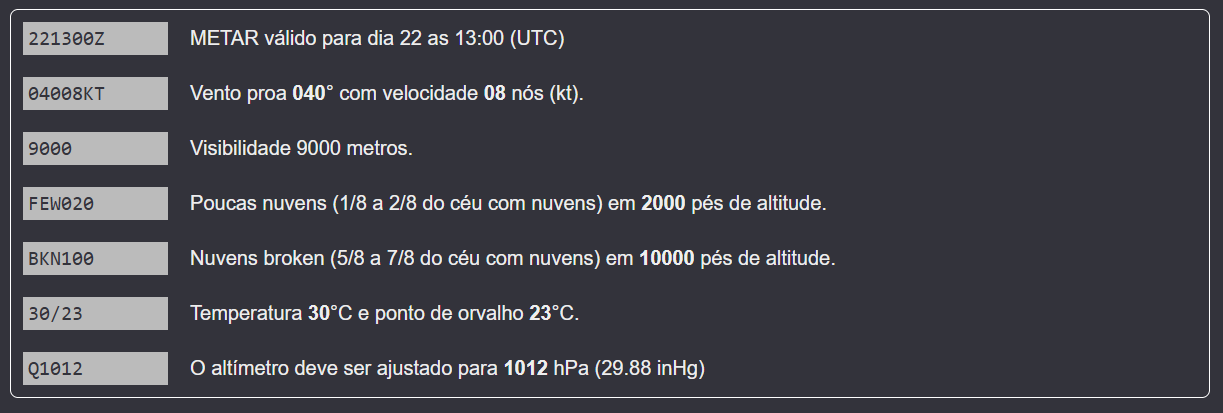
\includegraphics[width=0.8\linewidth]{img/METAR-SBBE.png}
        \label{fig:UI}
        \end{center}
    \end{figure}
\end{frame}

\begin{frame}{TAF}
    \footnotesize{\texttt{
220859Z 2212/2312 06006KT 9999 SCT040 TX34/2217Z TN24/2309Z \\
    BECMG 2215/2217 34013KT SCT040 FEW045TCU \\
    TEMPO 2220/2222 TS SCT030 FEW035CB \\
    BECMG 2222/2224 04008KT CAVOK \\
    BECMG 2310/2312 SCT020 RMK PGX}}

  \begin{figure}[ht]
    \begin{center}
    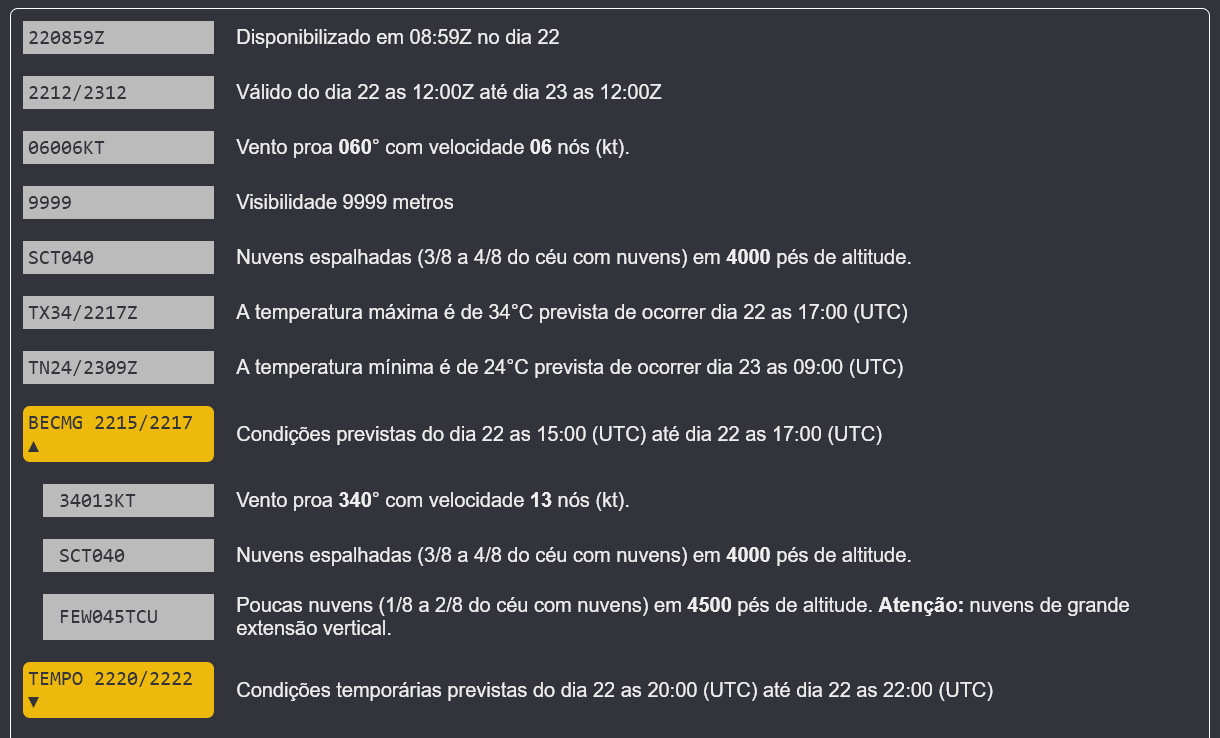
\includegraphics[width=0.7\linewidth]{img/TAF-SBBE.png}
    \label{fig:UI}
    \end{center}
    \end{figure}
\end{frame}

\begin{frame}{Histórico}
    \begin{itemize}
        \item TODO
    \end{itemize}
\end{frame}

\section{Teste de carga}

\section{Conclusão}

\begin{frame}{Conclusão}
    \begin{itemize}
        \item TODO
    \end{itemize}
\end{frame}

\begin{frame}{Obrigado}
    \centering
    \Huge Obrigado! \\
    \normalsize Perguntas?
\end{frame}

\end{document}

